\section{Ongoing developments}
The software framework and event reconstruction described in the previous sections is based on the code which is currently being utilized for data processing or near to be deployed. Nevertheless, as CLAS12 data are being analyzed, several potential improvements have been identified and are either in the process of being implemented or planned for the near future. In this section, we discussed the most relevant ones.

\begin{figure*}
\centering
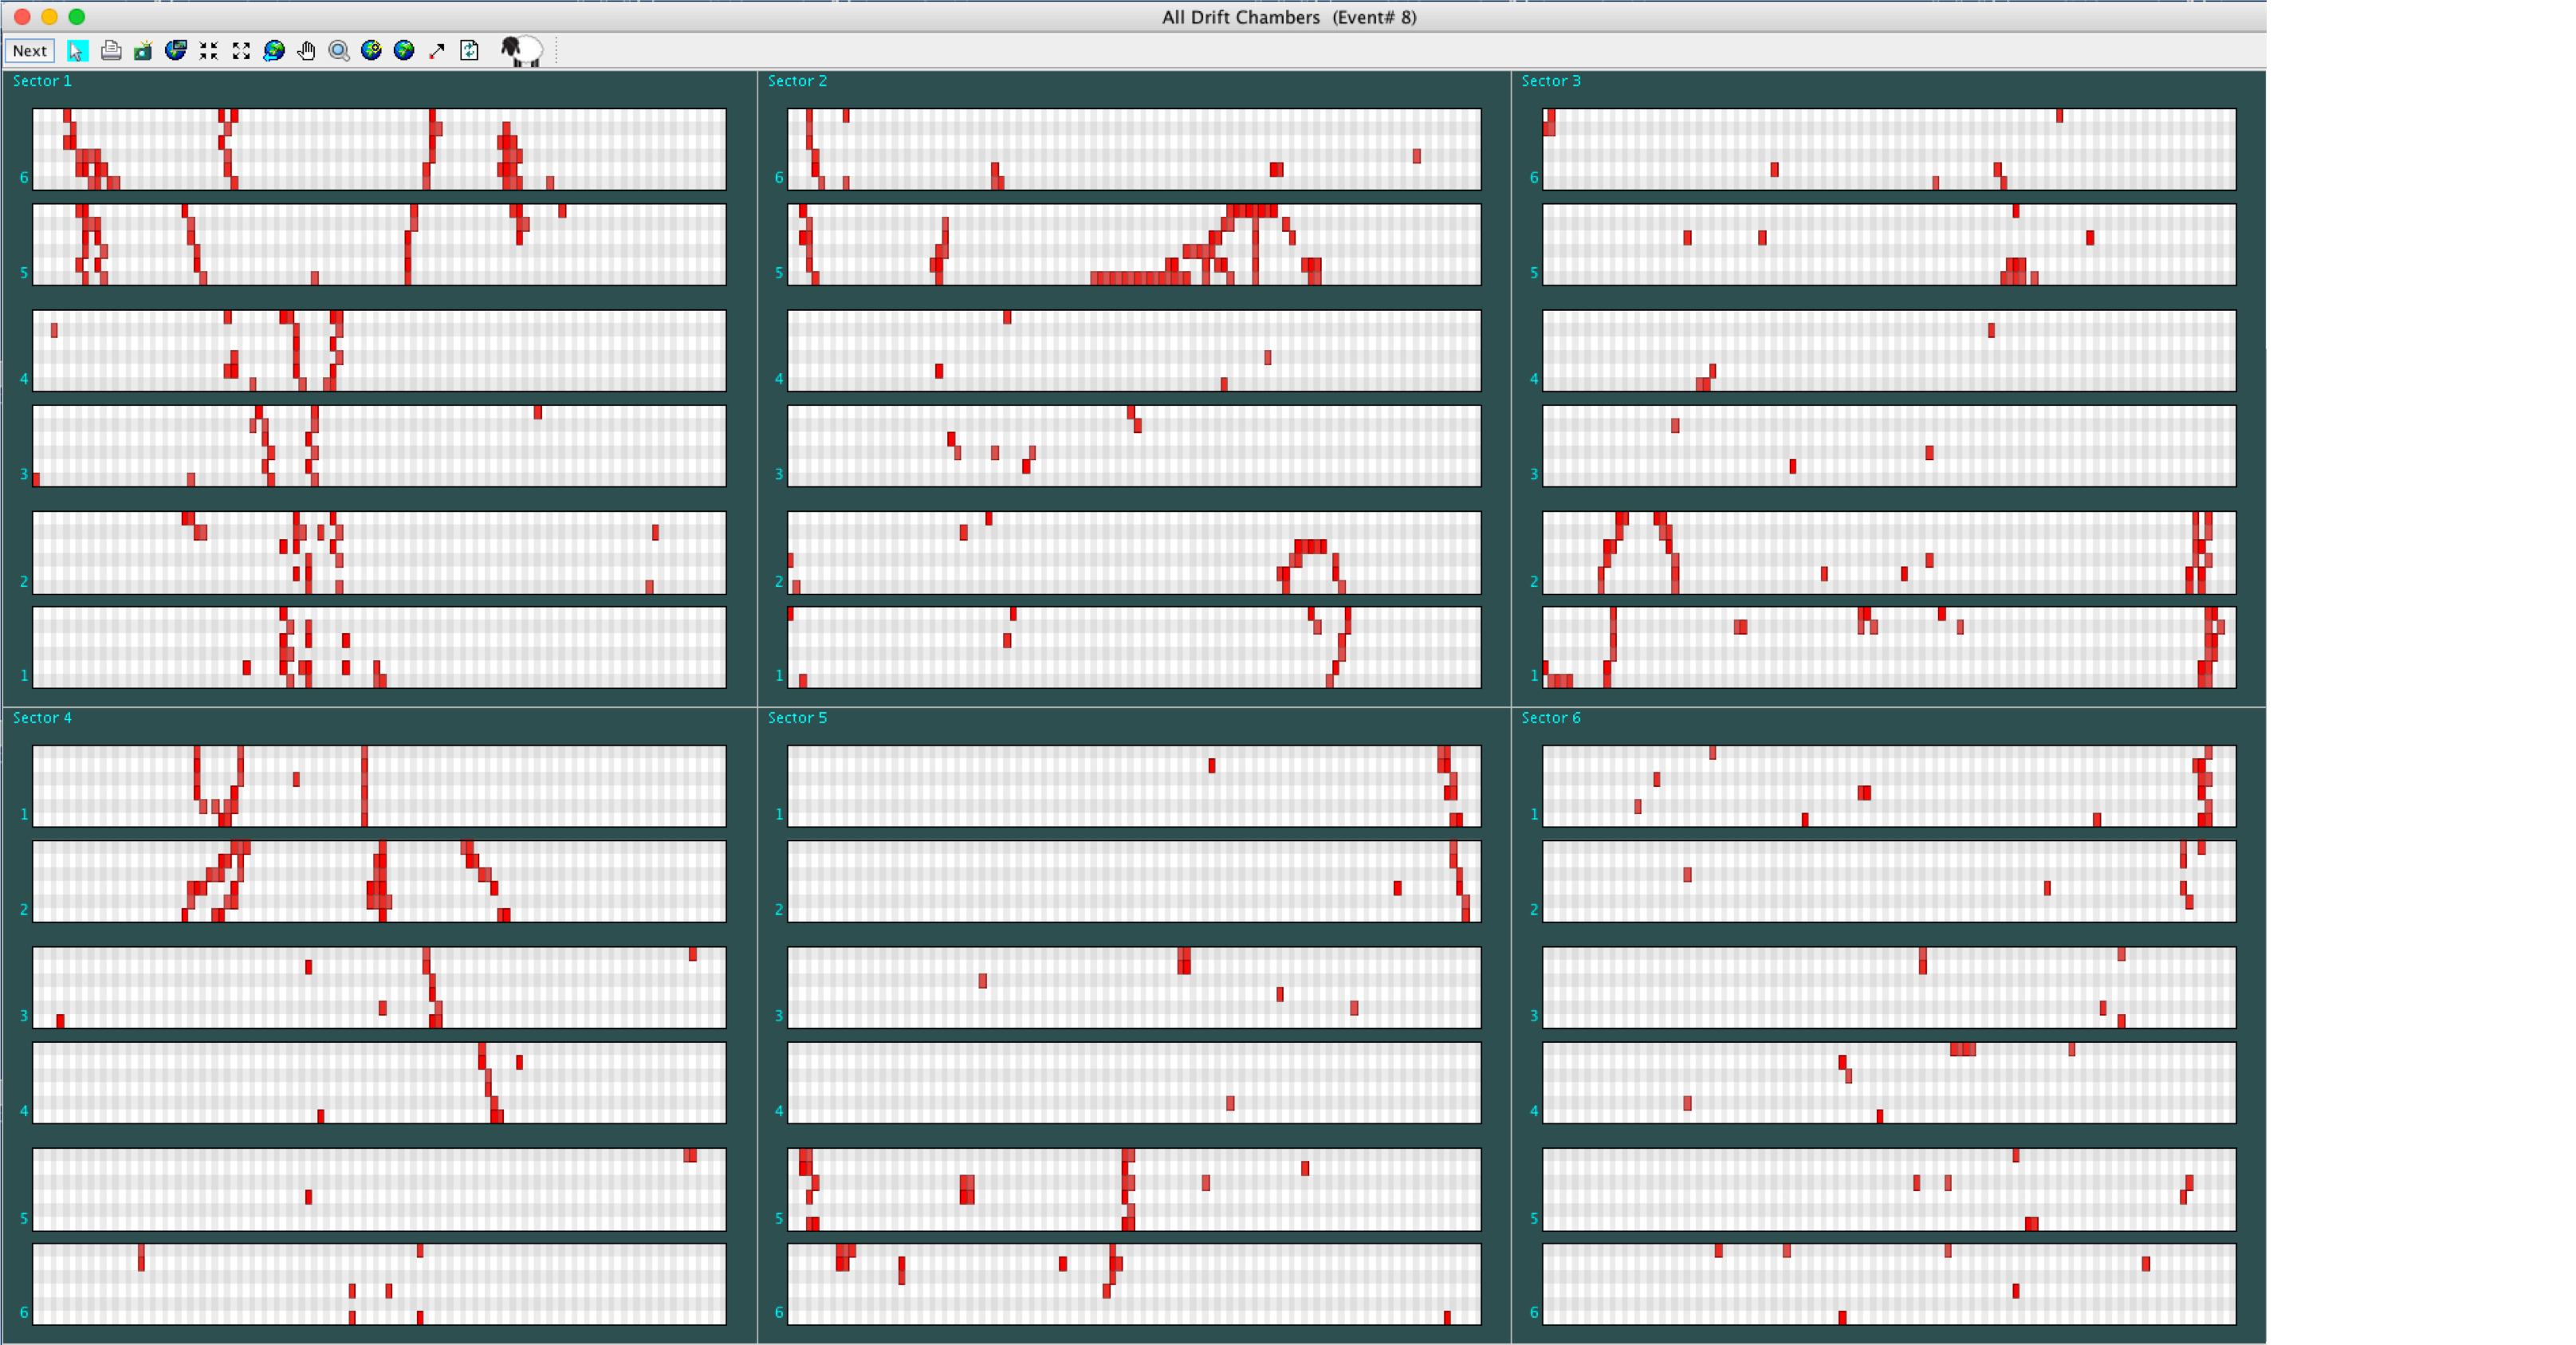
\includegraphics[width=0.95\textwidth]{pics/nn1.png}
\caption{Event display of track segments in the DC. 
}
\label{fig:nn1}
\end{figure*}
\subsection{Artificial Intelligence Assisted Forward Tracking}
Recent progress in machine learning field offer a promising alternative to conventional
algorithmic tracking methods. While the conventional
methods provide algorithms that are well understood and well studied, there are some algorithms
in data reconstruction process that can be substituted with neural networks to reduce data
processing times. For CLAS12, tracking is the most time consuming process in experimental data processing.
Tracking in the DC takes up to $\sim 90$\% of total data processing time, which includes finding
track candidates and iterating through track forming segments combinatorially to find the best
combinations of segments that can form a track. This time increases with luminosity as the number of noise
segments increases and can lead to processing time degradation with higher luminosity. We have started 
to address this issue by employing machine learning techniques to find best track candidates in
each event and reduce the number of combinatorics.

With increased luminosity the number of potential DC cross candidates
increases.  This implies that the  Kalman Filter fitting algorithm must be run for all possible
combinations crosses.  Fig.~\ref{fig:nn1} shows a typical example of drift
chamber data is shown in a longitudinal projective view using CED. 
This figure illustrates the potential of combinatorial trials to identify tracks. 
We are developing a classifier convolutional neural network that can
identify which segments from each region of CLAS12 drift chambers can potentially form a
good track. We intend to use this network in reconstruction process to reduce the number of
combinatorial fitting.
Reconstructed track segments from both positive and negative tracks from the currently reconstructed data samples are used to train the Neural Network. 
We are currently testing three types of Neural Networks: boosted decision tree, multilayer perceptron, convolutional neural network.  
The accuracy of the network is measured using 4 quantities:
\begin{itemize}
\item{The ratio of valid tracks (correctly detected) to the total number of tracks in the sample. }
\item{The ratio of valid tracks and  invalid tracks (miss-predicted as valid ones; i.e. False Positives) to the total number of tracks in the sample. }
\item{The ratio of valid tracks (correctly detected with highest probability) to the total number of tracks in the sample. }
\item{The ratio of invalid tracks (False Positives) to the total number of tracks in the sample. }
\end{itemize}
Accuracy scores were determined for different training set and for the 3 types of Neural Networks studied.  Preliminary results indicated that the Convolutional Neural Network performed competitively with the Multilayer Perceptron with about 97\% accuracy and 3\% False Positives. 

The hits identified as On-Track by the Neural Network are saved in a bank and the DC reconstruction package was adapted to read these data as an input to hit-based tracking.

Benchmark results of reconstruction speed for hit-based tracking are shown in Fig.~\ref{fig:nn2}

\begin{figure}
\centering
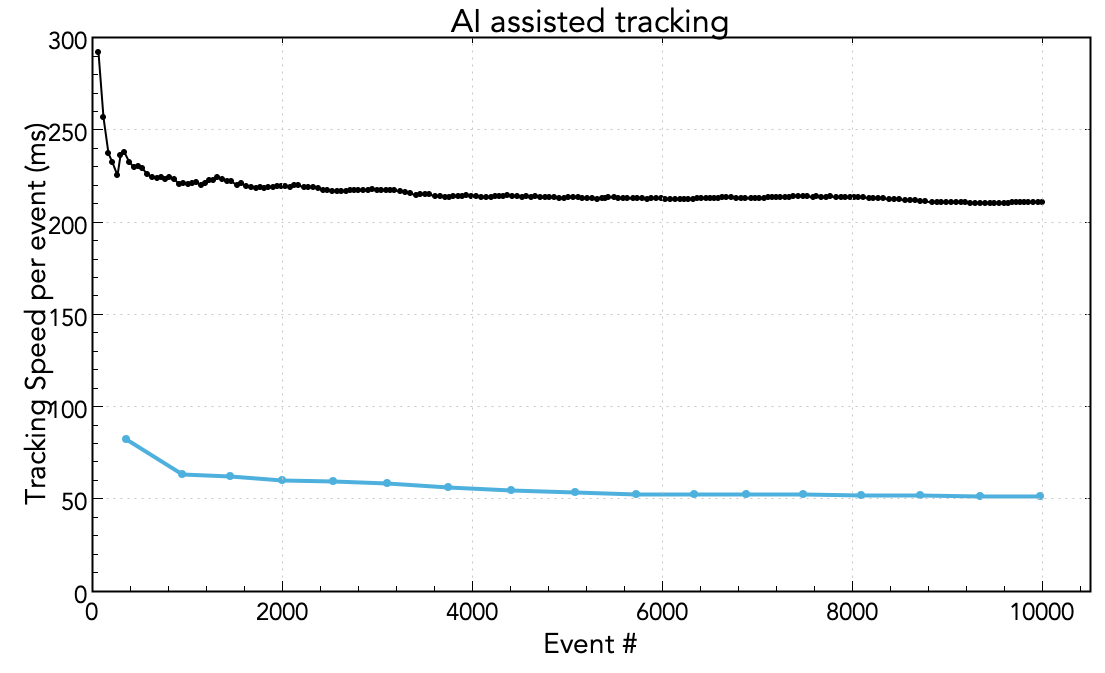
\includegraphics[width=0.45\textwidth]{pics/nn2.png}
\caption{Benchmark results of reconstruction speed for hit-based tracking.  
The (black) blue curve correspond to the (non) AI-assisted reconstruction processing time as a function of event number. 
}
\label{fig:nn2}
\end{figure}

The implementing the Neural Network software into the CLAS12 reconstruction workflow is under development. The second stage of the Machine Learning project will concentrate on efficiency improvements using AI-assisted tracking.

\subsection{Improvements to Central Tracking}
Improvements to tracking in the central detectors are currently being studied. These includes:
\begin{itemize}
    \item improvements to the geometry description of the detectors and fitting algorithm that remove systematic shifts that are currently observed in the fit residuals;
    \item implementation of geometrical distortions derived from detector alignment;
    \item use of the actual beam spot information in the initial fit of the track in the x-y plane;
    \item use of SVT clusters instead of crosses in the seeding.
\end{itemize}
The updates aim at enhancing the robustness of the tracking algorithm and improving resolution and efficiency.

\subsection{Improvements to Time-of-Flight reconstruction}
As discussed in Sec.~\ref{tof-sys}, the output of time-of-flight reconstruction that is currently passed to the event builder stage are reconstructed hits. Improvements in timing resolution for particles going through two adjacent paddles are expected using clusters. This is currently being studied on Monte Carlo simulations.

\subsection{Improvements to Event Builder}
The matching of tracks to detector responses, either hits or clusters, is currently based on the distance of closest approach between the tracks and the response coordinates. Improvements to this matching can be obtained using track trajectories, i.e. intersections of the track with the relevant detector planes were responses are reported, and timing information. The use of trajectories will reduce the uncertainty on the path length determination resulting for the resolution on the response coordinates. The use of timing information in the matching will reduce the effect of accidentals in high rates detectors such as the HTCC.


